\documentclass[10pt]{beamer}

\usetheme{m}

\usepackage{subcaption}
\usepackage{siunitx}
\usepackage{booktabs}
\usepackage[scale=2]{ccicons}

\usepackage{pgfplots}
\usepgfplotslibrary{dateplot}

\setlength\parindent{0pt}
\graphicspath{{./figures/}}
\newcommand{\norm}[1]{\left\lVert#1\right\rVert}

\title{Vibrating {\rmfamily\textsc{MEMS}} Gyroscopes}
\date{\today}
\author{Salah Missri}
\institute{EPFL}

\begin{document}

\maketitle

% \begin{frame}
%   \frametitle{Table of Contents}
%   \setbeamertemplate{section in toc}[sections numbered]
%   \tableofcontents[hideallsubsections]
% \end{frame}

% \section{Working principle}

\begin{frame}
\frametitle{Vibratory gyroscope: the Coriolis effect}
\begin{columns}
    \begin{column}{.48\textwidth}
        \begin{figure}
            \centering
            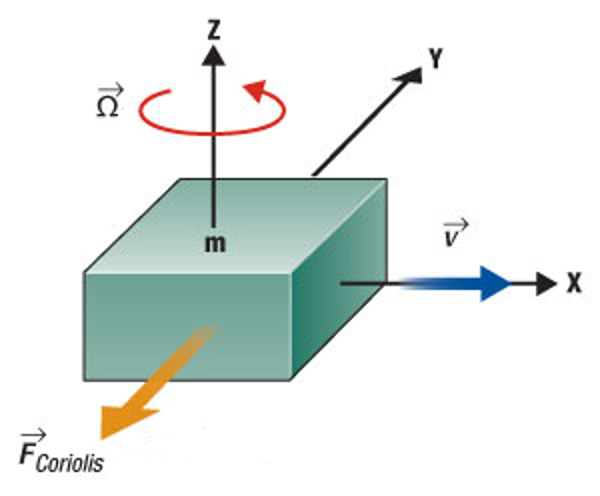
\includegraphics[width=1.\linewidth]{coriolis1.png}
            \caption{Coriolis effect on a mass\cite{MEMSblog}}
            \label{fig:coriolis}
        \end{figure}
    \end{column}
    \hfill
    \begin{column}{.60\textwidth}
        \begin{itemize}
            \item Coriolis force is proportional to the angular rate
            \begin{equation*}
                \mathbf{F_{Coriolis} = - 2 m \mathbf{\Omega} \times \mathbf{v}}
            \end{equation*}
            \item We can determine $F_{Coriolis}$ by measuring deflection (usually a capacitance measurement)
            \begin{equation*}
                \mathbf{\Omega} \propto \mathbf{F_{Coriolis}} \to \mathbf{F} \propto \mathbf{x} \propto \mathbf{C}
            \end{equation*}
            \item But this will also measure linear acceleration
            \begin{equation*}
                \mathbf{F \neq F_{Coriolis}}
            \end{equation*}
        \end{itemize}
    \end{column}
\end{columns}
\end{frame}

\begin{frame}
\frametitle{Vibratory gyroscope: theory of operation}
    Consider that the fig.\ref{fig:coriolis} system is oscillating purely in the x-axis at resonant frequency $\omega_r$ ($\mathbf{v} = A_x \omega_r \cos{(\omega_r t)} \mathbf{e_x}$) is submitted to angular rotation in input axis $\mathbf{\Omega} = \Omega_z \mathbf{e_z}$
    \begin{equation*}
        \norm{\mathbf{F_{Coriolis}}} = 2 m \Omega_z A_x \omega_r \cos{(\omega_r t)}
    \end{equation*}

    Considering the mass is attached to springs along x and y axes, the Coriolis force generates a deflection in the y-axis $\mathbf{F_{Coriolis}} = k_y \Delta y$.
    \begin{equation*}
        \Delta y = \frac{F_{Coriolis}}{k_y} = \frac{2 m \Omega_z A_x \omega_r \cos{(\omega_r t)}}{k_y}
    \end{equation*}

    This can be measured through capacitance: $C = \frac{\epsilon S}{y_0 + \Delta y} \sim \epsilon S (y_0 - \Delta y)$.
\end{frame}

\begin{frame}
\frametitle{Tuning fork gyroscope (1/2)}
\begin{columns}
    \begin{column}{.48\textwidth}
        \begin{figure}
        \centering
            \begin{subfigure}[t]{0.9\textwidth}
                \centering
                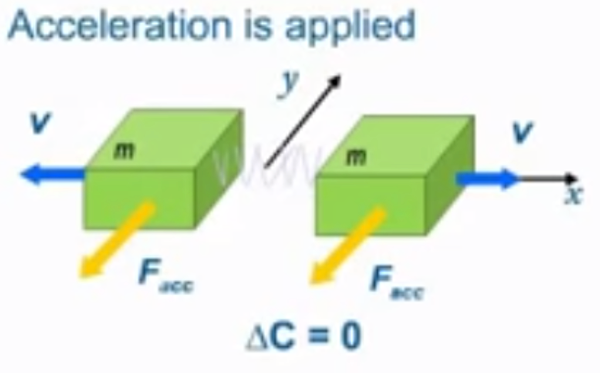
\includegraphics[width=\linewidth]{GyroAcc.png}
            \end{subfigure}
            ~
            \begin{subfigure}[t]{0.9\textwidth}
                \centering
                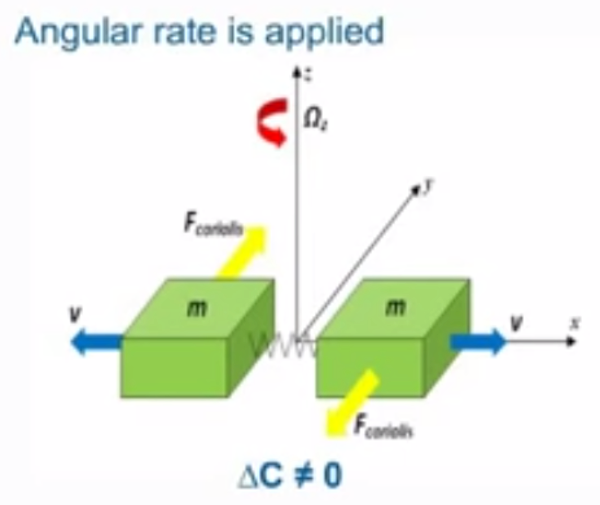
\includegraphics[width=\linewidth]{GyroAngRate.png}
            \end{subfigure}
        \caption{Tuning fork configuration}
        \end{figure}
    \end{column}
    \hfill
    \begin{column}{.60\textwidth}
        \begin{itemize}
            \item Using two coupled masses vibrating in antiphase (tuning fork configuration)
            \begin{equation*}
                \mathbf{F_{Coriolis, 1}} = - 2 m \mathbf{\omega} \times \mathbf{v} = \mathbf{F_{Coriolis, 2}}
            \end{equation*}
            \item Measure the difference between the two masses
            \begin{equation*}
                \mathbf{\omega} \propto \mathbf{F_{Coriolis}} \propto \Delta \mathbf{F} \propto \Delta \mathbf{x} \propto \Delta \mathbf{C}
            \end{equation*}
            \item Isolates Coriolis force measurement from linear acceleration
        \end{itemize}
    \end{column}
\end{columns}
\end{frame}

\begin{frame}
\frametitle{Tuning fork gyroscope (2/2)}
\begin{columns}
    \begin{column}{.45\textwidth}
        \begin{figure}
            \centering
            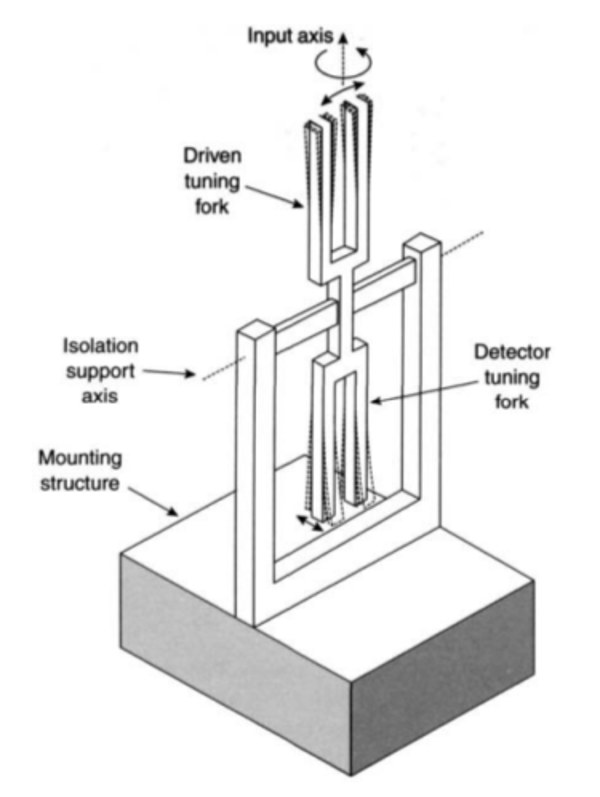
\includegraphics[width=0.9\linewidth]{quartz_rate_gyro.png}
            \caption{Quartz rate sensor\cite{Titterton}}
        \end{figure}
    \end{column}
    \hfill
    \begin{column}{.70\textwidth}
        \begin{figure}
            \centering
            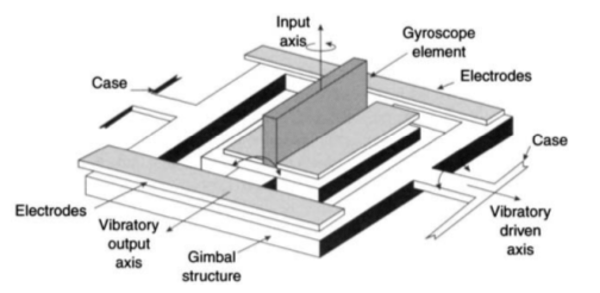
\includegraphics[width=1.0\linewidth]{silicon_gyro.png}
            \caption{1D MEMS gyroscope\cite{Titterton}}
        \end{figure}
    \end{column}
\end{columns}
\end{frame}

% \section{Limitations}

\begin{frame}
\frametitle{Limitations}
    For the single 1D sensors
    \begin{itemize}
        \item Sensitive to change in ambient temperature
    \end{itemize}

    For 3D sensing using 1D sensors
    \begin{itemize}
        \item Alignement issues (getting the sensors at exactly $90^{\circ}$)
        \item Getting the same vibration frequency for all three masses
        \item Cross-talk particularly if all three sensors are on the same substrate (also present if other types of vibrating sensors are used)
    \end{itemize}
\end{frame}

\begin{frame}
\frametitle{Multi-axis gyroscope sensors}
\begin{columns}
    \begin{column}{.58\textwidth}
        \begin{figure}
            \centering
            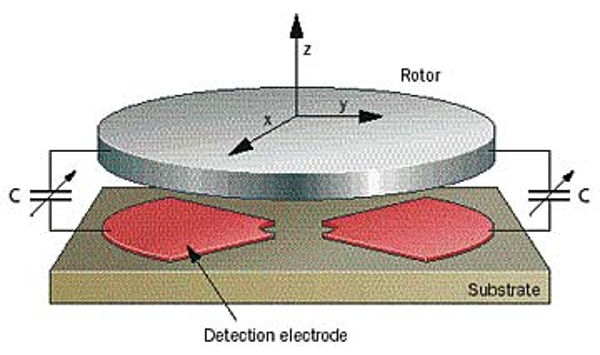
\includegraphics[width=1.0\linewidth]{vibrating_disk.png}
            \caption{Vibrating disk gyroscope (2D)\cite{Bosch}}
        \end{figure}
    \end{column}
    \hfill
    \begin{column}{.48\textwidth}
        \begin{figure}
            \centering
            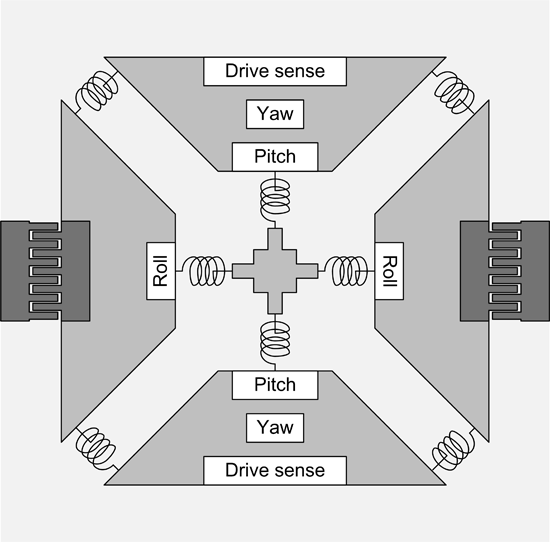
\includegraphics[width=1.0\linewidth]{gyro_mems_3in1.png}
            \caption{3D MEMS gyroscope\cite{ST}}
        \end{figure}
    \end{column}
\end{columns}
\end{frame}

% \section{Advantages \& drawbacks}

\begin{frame}
\frametitle{Advantages}
    \begin{itemize}
        \item Can be made rugged to resist very high accelerations ($> 10000$ g)
        \item Very short reaction time (i.e. rapid start-up capability)
        \item Good shelf life and dormancy (because no bearings or lubricants)
        \item Low power consumption
        \item Small
    \end{itemize}
\end{frame}

\begin{frame}
\frametitle{Drawbacks}
    \begin{itemize}
        \item High bias ($0.1$ to $1^{\circ}$/s)
        \item Sensitivity to environment effects
        \begin{itemize}
            \item Temperature changes
            \item Vibratory motion (cross-talk)
        \end{itemize}
    \end{itemize}
\end{frame}

% \section{Performances \& applications}
\begin{frame}
\frametitle{Performances}
    \begin{table}
    \begin{tabular}{lr}
        \toprule
        Bandwidth                   & 0 to \SI{500}{\hertz} \\
        Dynamic range               & $\pm 10$ to $\pm \SI{1000}{\degree/\second}$ \\
        Resolution                  & $< \SI{0.1}{\degree/\second}$ \\
        Bias                        & $0.1$ to \SI{1}{\degree/\second} \\
        Error due to temperature    & $0.01$ to \SI{0.05}{\%/\celsius} \\
        Shock resistance            & $> \SI{20000}{g}$ \\
        Cost                        & 1 to \SI{10}{\$} \\
        \bottomrule
    \end{tabular}
    \caption{Typical performances}
    \end{table}
\end{frame}

\begin{frame}
\frametitle{Applications}
    Not good enough for inertial navigation systems, but good enough for control and stabilisation processes
    \begin{itemize}
        \item Automobile: driving assistance (skid and roll prevention)
        \item Robotics
        \begin{itemize}
            \item Inertial navigation on small autonomous systems
            \item Control and stabilisation
        \end{itemize}
        \item Motion sensing in smartphones and entertainment devices (Wii)
    \end{itemize}
\end{frame}

% \section{References}

\begin{frame}[allowframebreaks]
\frametitle{References}
    \bibliography{presentation}
    \bibliographystyle{abbrv}
\end{frame}

\plain{Thank you for your attention\\Questions?}


\end{document}
